
\documentclass{article}

\usepackage[]{todonotes}
\usepackage[outdir=./]{epstopdf}
\usepackage[ruled]{algorithm2e}

\title{Parallel Standard Particle Swarm Optimization}
\author{Gian M. Fritsche}
\date{\today}

\begin{document}
	\maketitle

	\section{Introduction}

	The Particle Swarm Optimization~\cite{PSO95} is a meta-heuristic based on the behaviour of bird flocks. Every iteration, each particle moves on the search space based on three components.

	\begin{itemize}
		\item {\em Social:} This component contributes for the exploitation of the algorithm.
		It guides the search towards the best solutions found by the swarm.
		\item {\em Individual:} The individual component guides the particle to the best solution that the particle have found.
		\item {\em Inertia:} The inertia component increase the exploration of the algorithm. It is responsible for keep the particle moving towards an previous direction and avoid abrupt changes of direction.
	\end{itemize}

	The position of one particle is a set of variable values, {\em i.e.} a solution for an optimization problem. That solution is then evaluated and is associated to a fitness value. Based on the fitness value the Social and Individual components are updated.
	And finally, these components are used to compute the next position of the particle (another solution for the problem).

	Since its first publication several adaptations and improvements have been proposed.
	In 2006 it was created the first version of a Standard Particle Swarm Optimization~\cite{SPSO}. The objective was not propose the best PSO available, but establish a common benchmark as a baseline to assess the PSO variants in the literature.

	\subsection {Standard Particle Swarm optimization}

	Since its first publication (2006), there is three versions of SPSO: 2006, 2007 and 2011.
	In the latest version the description is given as follow:
	The first population (set of solutions) is initialized randomly in the search space. The velocity is also initialized randomly. The suggested population size is $40$. The neighbourhood topology used to update the social component is the Adaptive Random Topology (ART).
	In the ART each particle informs its current fitness to $K$ neighbours. If the fitness is better than the previous social best information of the neighbour the social best (fitness and position) is updated. The neighbourhood is defined by a directed graph where each particle informs its quality to (at most) $K$ neighbours. The graph is generated randomly initially and every time that the best global fitness is not improved.

	In the previous versions of PSO the velocity was updated dimension by dimension.
	But, in SPSO2011 the velocity is updated in a geometrical way,  that does not depend on the system of coordinates.

	\begin{algorithm}[H]
		\KwData{this text}
		\KwResult{how to write algorithm with \LaTeX2e }
		initialization\;
		\While{not at end of this document}{
		read current\;
		\eIf{understand}{
		go to next section\;
		current section becomes this one\;
		}{
		go back to the beginning of current section\;
		}
		}
		\caption{Standard Particle Swarm Optimization 2011}
	\end{algorithm}

	\section{Parallel Standard Particle Swarm Optimization}

	In this work we use the SPSO2011.

	\todo[inline]{Parallel SPSO2011 description}
	\todo[inline]{Parallel SPSO2011 pseudo-code}
	\todo[inline]{Parallel SPSO2011 characteristics (shared memory, warp size, multi-blocks)}

	\section{Experiments and Results}

	\begin{figure}[!htb]
		\centering
		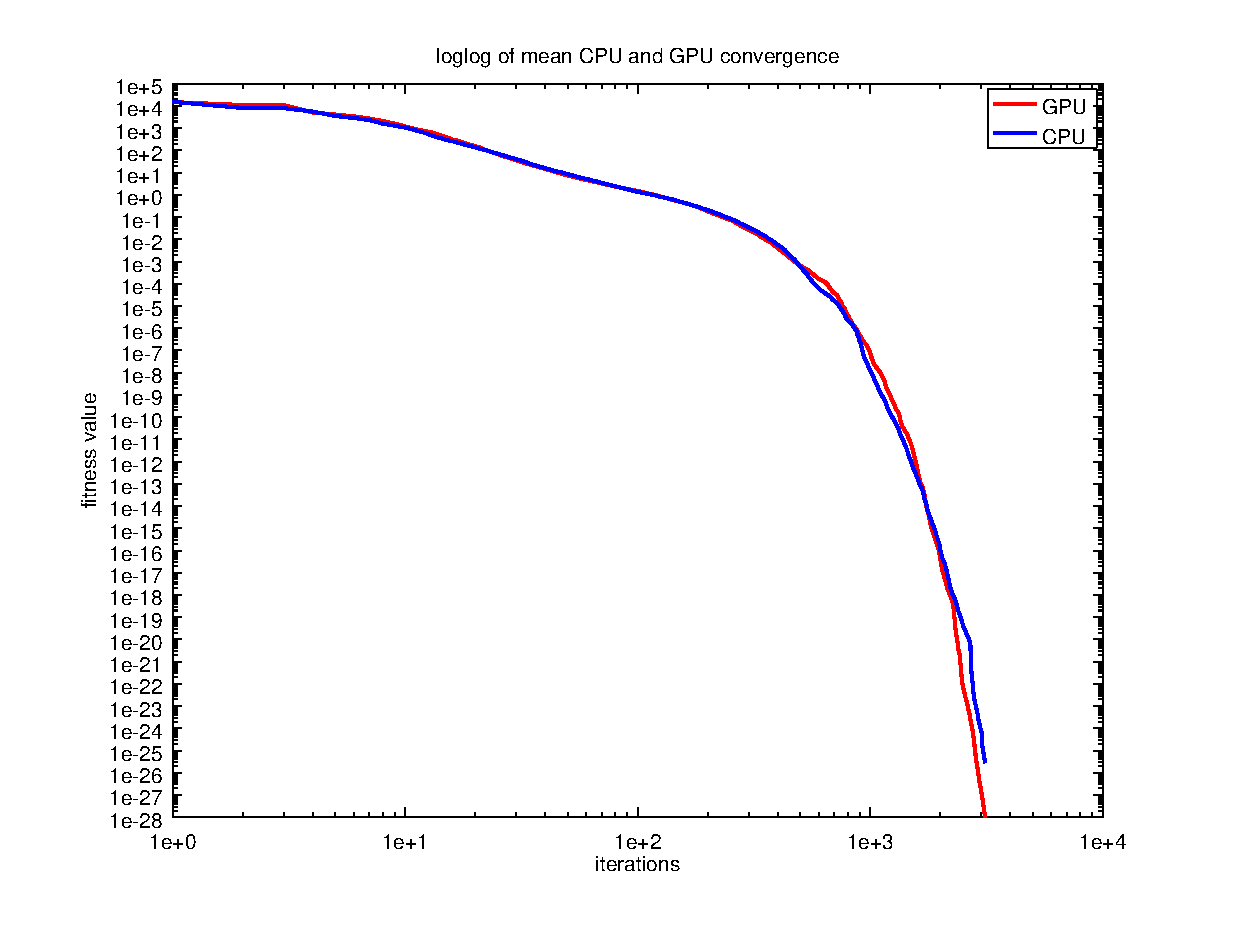
\includegraphics[width=.8\textwidth]{../img/loglog_convergence.eps}
		\caption{loglog of mean CPU and GPU convergence}
		\label{fig:loglog_convergence}
	\end{figure}

	\begin{figure}[!htb]
		\centering
		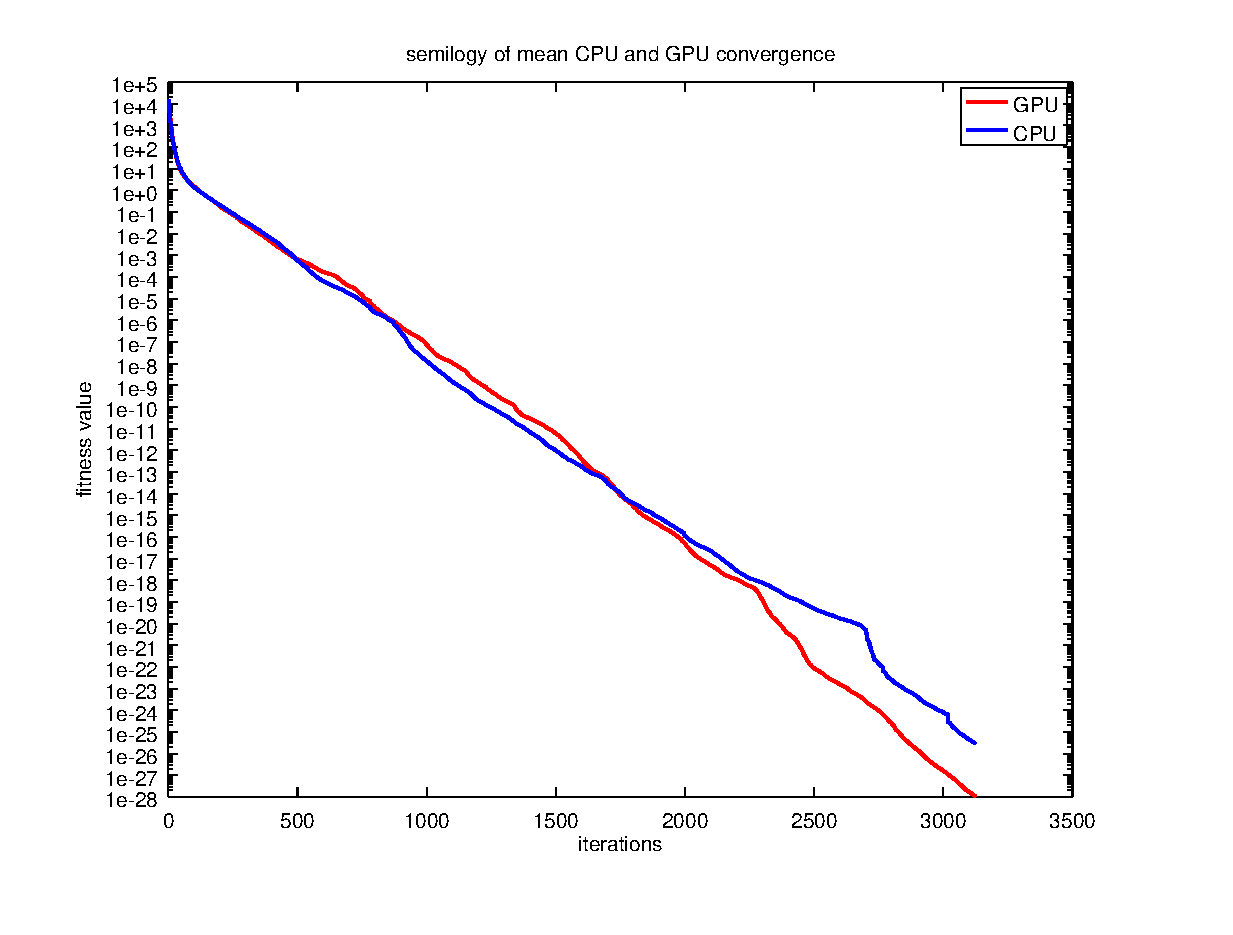
\includegraphics[width=.8\textwidth]{../img/semilogy_convergence.eps}
		\caption{semilogy of mean CPU and GPU convergence}
		\label{fig:semilogy_convergence}
	\end{figure}


	\begin{figure}[!htb]
		\centering
		\includegraphics[width=.8\textwidth]{../img/sphere10_32particles_fitness.eps}
		\caption{semilogy of mean CPU and GPU convergence}
		\label{fig:semilogy_convergence}
	\end{figure}


	\begin{figure}[!htb]
		\centering
		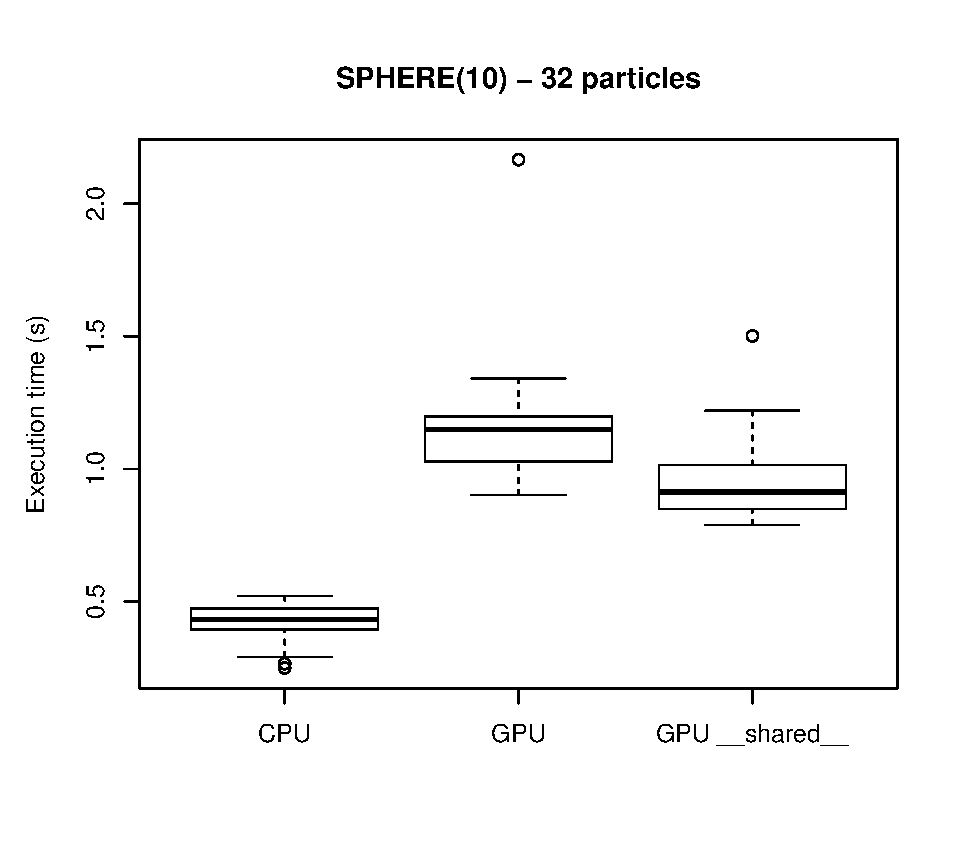
\includegraphics[width=.8\textwidth]{../img/sphere10_32particles_time.eps}
		\caption{semilogy of mean CPU and GPU convergence}
		\label{fig:semilogy_convergence}
	\end{figure}

	\begin{figure}[!htb]
		\centering
		\includegraphics[width=.8\textwidth]{../img/sphere10_32particles_multi_runs_fitness.eps}
		\caption{semilogy of mean CPU and GPU convergence}
		\label{fig:semilogy_convergence}
	\end{figure}


	\begin{figure}[!htb]
		\centering
		\includegraphics[width=.8\textwidth]{../img/sphere10_32particles_multi_runs_time.eps}
		\caption{semilogy of mean CPU and GPU convergence}
		\label{fig:semilogy_convergence}
	\end{figure}

	

	\section{Conclusions}

	\bibliographystyle{plain}
	\bibliography{bibliography} 

\end{document}
